\section{Условие}

В информационный центр приходят клиенты через интервал времени 10 $\pm$ 2 минуты. Если все три имеющихся оператора заняты, клиенту отказывают в обслуживании. Операторы имеют разную производительность и могут обеспечивать обслуживание среднего запроса пользователя за 20 $\pm$ 5; 40 $\pm$ 10; 40 $\pm$ 20. Клиенты стремятся занять свободного оператора с максимальной производительностью. Полученные запросы сдаются в накопитель. Откуда выбираются на обработку. На первый компьютер запросы от 1 и 2-ого операторов, на второй -- запросы от 3-его. Время обработки запросов первым и 2-м компьютером равны соответственно 15 и 30 мин. Промоделировать процесс обработки 300 запросов. Определить вероятность отказа.

\section{Теория}

На рисунке \ref{fig:model} представлена структурная схема  данной концептуальной модели.

\begin{figure}[H]
    \centering
    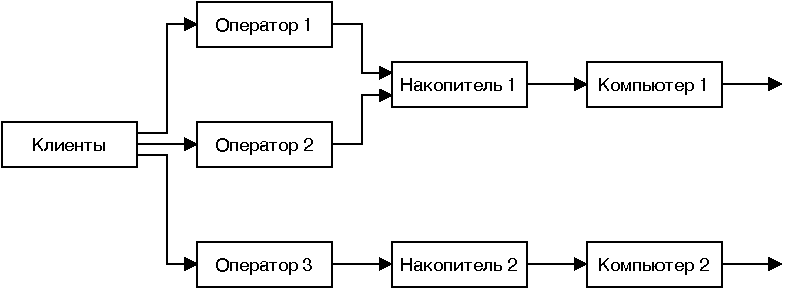
\includegraphics[width=0.9\textwidth]{img/content/model.pdf}
    \caption{Структурная схема}
    \label{fig:model}
\end{figure}

Поскольку значение требующейся в условии вероятности отказа находится в промежутке, то необходимо смоделировать систему много раз.

\section{Результаты}

На рисунке \ref{fig:result} представлен результат полученный путем 1000 моделирований системы.

\begin{figure}[H]
    \centering
    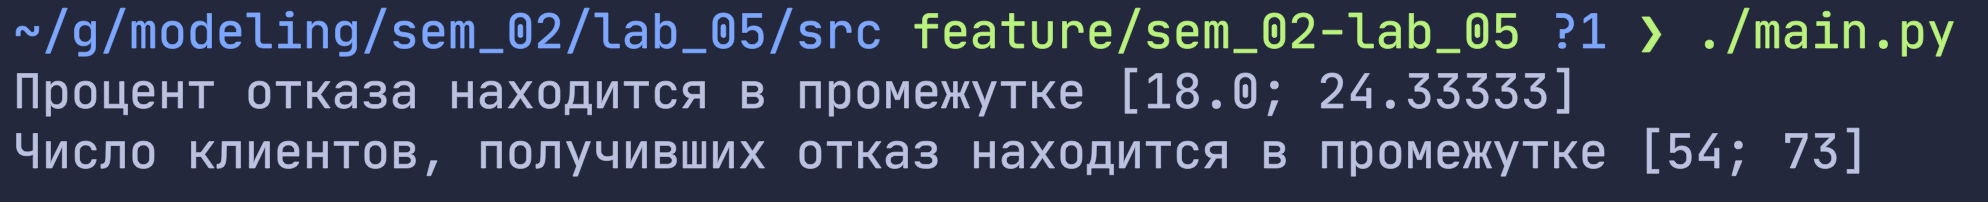
\includegraphics[width=0.8\textwidth]{img/content/result.png}
    \caption{Полученный результат}
    \label{fig:result}
\end{figure}

\section{Вывод}

Разработана программа, результатом работы которой являются промежутки, в которых находились значения вероятности отказа и количества отказов, полученных в результате 1000 моделирований системы.
